%-----------------------------------------------------------------------------------------------------------------------------------------------%
%	The MIT License (MIT)
%
%	Copyright (c) 2019 Jan Küster
%	Modified 2023 by Thomas Phil
%
%	Permission is hereby granted, free of charge, to any person obtaining a copy
%	of this software and associated documentation files (the "Software"), to deal
%	in the Software without restriction, including without limitation the rights
%	to use, copy, modify, merge, publish, distribute, sublicense, and/or sell
%	copies of the Software, and to permit persons to whom the Software is
%	furnished to do so, subject to the following conditions:
%	
%	THE SOFTWARE IS PROVIDED "AS IS", WITHOUT WARRANTY OF ANY KIND, EXPRESS OR
%	IMPLIED, INCLUDING BUT NOT LIMITED TO THE WARRANTIES OF MERCHANTABILITY,
%	FITNESS FOR A PARTICULAR PURPOSE AND NONINFRINGEMENT. IN NO EVENT SHALL THE
%	AUTHORS OR COPYRIGHT HOLDERS BE LIABLE FOR ANY CLAIM, DAMAGES OR OTHER
%	LIABILITY, WHETHER IN AN ACTION OF CONTRACT, TORT OR OTHERWISE, ARISING FROM,
%	OUT OF OR IN CONNECTION WITH THE SOFTWARE OR THE USE OR OTHER DEALINGS IN
%	THE SOFTWARE.
%	
%
%-----------------------------------------------------------------------------------------------------------------------------------------------%


%============================================================================%
%
%	DOCUMENT DEFINITION
%
%============================================================================%

%we use article class because we want to fully customize the page and don't use a cv template
\documentclass[A4]{article}	
\usepackage[fontsize=9pt]{fontsize}

\usepackage{bibentry}
\makeatletter\let\saved@bibitem\@bibitem\makeatother
\usepackage{apacite}

\renewcommand{\doiprefix}{}

%----------------------------------------------------------------------------------------
%	ENCODING
%----------------------------------------------------------------------------------------

% we use utf8 since we want to build from any machine
\usepackage[utf8]{inputenc}		

%----------------------------------------------------------------------------------------
%	LOGIC
%----------------------------------------------------------------------------------------

% provides \isempty test
\usepackage{xstring, xifthen}

%----------------------------------------------------------------------------------------
%	FONT BASICS
%----------------------------------------------------------------------------------------

% some tex-live fonts - choose your own

%\usepackage[defaultsans]{droidsans}
%\usepackage[default]{comfortaa}
%\usepackage{cmbright}
%\usepackage[default]{raleway}
%\usepackage[default]{raleway}
%\usepackage[condensed,thin]{roboto}
%\usepackage[]{inconsolata}
%\usepackage[frenchstyle]{kpfonts}
%\usepackage{fetamont}
%\usepackage[default]{gillius}
%\usepackage[light,math]{iwona}

%\usepackage[]{inconsolata}
\usepackage[scaled=1.01]{helvet}
%\usepackage[light]{FiraSans}
\usepackage[letterspace=100]{microtype}

% set font default
\renewcommand*\familydefault{\sfdefault} 	
\usepackage[T1]{fontenc}

% more font size definitions
\usepackage{moresize}

%----------------------------------------------------------------------------------------
%	FONT AWESOME ICONS
%---------------------------------------------------------------------------------------- 

% include the fontawesome icon set
\usepackage{fontawesome}

% use to vertically center content
% credits to: http://tex.stackexchange.com/questions/7219/how-to-vertically-center-two-images-next-to-each-other
\newcommand{\vcenteredinclude}[1]{\begingroup
\setbox0=\hbox{\includegraphics{#1}}%
\parbox{\wd0}{\box0}\endgroup}

% use to vertically center content
% credits to: http://tex.stackexchange.com/questions/7219/how-to-vertically-center-two-images-next-to-each-other
\newcommand*{\vcenteredhbox}[1]{\begingroup
\setbox0=\hbox{#1}\parbox{\wd0}{\box0}\endgroup}

% icon shortcut
\newcommand{\icon}[3] { 							
	\makebox(#2, #2){\textcolor{maincol}{\csname fa#1\endcsname}}
}	

% icon with text shortcut
\newcommand{\icontext}[4]{ 						
	\vcenteredhbox{\icon{#1}{#2}{#3}}  \hspace{2pt}  \parbox{0.9\mpwidth}{\textcolor{#4}{#3}}
}

% icon with website url
\newcommand{\iconhref}[5]{ 						
    \vcenteredhbox{\icon{#1}{#2}{#5}}  \hspace{2pt} \href{#4}{\textcolor{#5}{#3}}
}

% icon with email link
\newcommand{\iconemail}[5]{ 						
    \vcenteredhbox{\icon{#1}{#2}{#5}}  \hspace{2pt} \href{mailto:#4}{\textcolor{#5}{#3}}
}

% icon with linkedin url
\newcommand{\iconlinkedin}[5]{ 						
	\vcenteredhbox{\icon{#1}{#2}{#5}}  \hspace{2pt} \href{#4}{\textcolor{#5}{#3}}
}


%----------------------------------------------------------------------------------------
%	PAGE LAYOUT  DEFINITIONS
%----------------------------------------------------------------------------------------

% page outer frames (debug-only)
% \usepackage{showframe}		

% we use paracol to display breakable two columns
\usepackage{paracol}

% define page styles using geometry
\usepackage[a4paper]{geometry}

% remove all possible margins
\geometry{top=.8cm, bottom=.8cm, left=.8cm, right=.8cm}

\usepackage{fancyhdr}
\pagestyle{empty}

% space between header and content
% \setlength{\headheight}{0pt}

% indentation is zero
\setlength{\parindent}{0mm}

%----------------------------------------------------------------------------------------
%	TABLE /ARRAY DEFINITIONS
%---------------------------------------------------------------------------------------- 

% extended aligning of tabular cells
\usepackage{array}

% custom column right-align with fixed width
% use like p{size} but via x{size}
\newcolumntype{x}[1]{%
>{\raggedleft\hspace{0pt}}p{#1}}%


%----------------------------------------------------------------------------------------
%	GRAPHICS DEFINITIONS
%---------------------------------------------------------------------------------------- 

%for header image
\usepackage{graphicx}

% use this for floating figures
% \usepackage{wrapfig}
% \usepackage{float}
% \floatstyle{boxed} 
% \restylefloat{figure}

%for drawing graphics		
\usepackage{tikz}				
\usetikzlibrary{shapes, backgrounds,mindmap, trees}

%----------------------------------------------------------------------------------------
%	Color DEFINITIONS
%---------------------------------------------------------------------------------------- 
\usepackage{transparent}
\usepackage{color}

% primary color
%\definecolor{maincol}{RGB}{ 225, 0, 0 }
\definecolor{maincol}{RGB}{ 69, 123, 157 }

% accent color, secondary
% \definecolor{accentcol}{RGB}{ 250, 150, 10 }
\definecolor{accentcol}{RGB}{ 81, 84, 95 }

% dark color
%\definecolor{darkcol}{RGB}{ 70, 70, 70 }
\definecolor{darkcol}{RGB}{ 69, 123, 157 }

% light color
%\definecolor{lightcol}{RGB}{245,245,245}
\definecolor{lightcol}{RGB}{ 168, 218, 220 }

\definecolor{textcol}{RGB}{ 39, 39, 39 }

\usepackage{xcolor}

\makeatletter
\newcommand{\globalcolor}[1]{%
	\color{#1}\global\let\default@color\current@color
}
\makeatother

\AtBeginDocument{\globalcolor{textcol}}

% Package for links, must be the last package used
\usepackage[hidelinks]{hyperref}
\makeatletter\let\@bibitem\saved@bibitem\makeatother

% returns minipage width minus two times \fboxsep
% to keep padding included in width calculations
% can also be used for other boxes / environments
\newcommand{\mpwidth}{\linewidth-\fboxsep-\fboxsep}
	


%============================================================================%
%
%	CV COMMANDS
%
%============================================================================%

%----------------------------------------------------------------------------------------
%	 CV LIST
%----------------------------------------------------------------------------------------

% renders a standard latex list but abstracts away the environment definition (begin/end)
\newcommand{\cvlist}[1] {
	\begin{itemize}{\setlength\itemsep{-.4em}#1}\end{itemize}
}

%----------------------------------------------------------------------------------------
%	 CV TEXT
%----------------------------------------------------------------------------------------

% base class to wrap any text based stuff here. Renders like a paragraph.
% Allows complex commands to be passed, too.
% param 1: *any
\newcommand{\cvtext}[1] {
	\begin{tabular*}{1\mpwidth}{p{0.98\mpwidth}}
		\parbox{1\mpwidth}{#1}
	\end{tabular*}
}

%----------------------------------------------------------------------------------------
%	CV SECTION
%----------------------------------------------------------------------------------------

% Renders a a CV section headline with a nice underline in main color.
% param 1: section title
\newcommand{\cvsection}[1] {
	\vspace{10pt}
	\cvtext{
		\textbf{\LARGE{\textcolor{darkcol}{\uppercase{#1}}}}\\[-4pt]
		\textcolor{maincol}{ \rule{0.1\textwidth}{2pt} } \\
	}
}

%----------------------------------------------------------------------------------------
%	META SKILL
%----------------------------------------------------------------------------------------

% Renders a progress-bar to indicate a certain skill in percent.
% param 1: name of the skill / tech / etc.
% param 2: level (for example in years)
% param 3: percent, values range from 0 to 1
\newcommand{\cvskill}[3] {
	\begin{tabular*}{1\mpwidth}{p{0.72\mpwidth}  r}
 		\textcolor{black}{\textbf{#1}} & \textcolor{maincol}{#2}\\
	\end{tabular*}%
	
	\hspace{4pt}
	\begin{tikzpicture}[scale=1,rounded corners=2pt,very thin]
		\fill [lightcol] (0,0) rectangle (1\mpwidth, 0.15);
		\fill [maincol] (0,0) rectangle (#3\mpwidth, 0.15);
  	\end{tikzpicture}%
}


%----------------------------------------------------------------------------------------
%	 CV EVENT
%----------------------------------------------------------------------------------------

% Renders a table and a paragraph (cvtext) wrapped in a parbox (to ensure minimum content
% is glued together when a pagebreak appears).
% Additional Information can be passed in text or list form (or other environments).
% the work you did
% param 1: time-frame i.e. Sep 14 - Jan 15 etc.
% param 2:	 event name (job position etc.)
% param 3: Customer, Employer, Industry
% param 4: Short description
% param 5: work done (optional)
% param 6: technologies include (optional)
% param 7: achievements (optional)
\newcommand{\cvevent}[7] {
	
	% we wrap this part in a parbox, so title and description are not separated on a pagebreak
	% if you need more control on page breaks, remove the parbox
	\parbox{\mpwidth}{
		\begin{tabular*}{1\mpwidth}{p{0.72\mpwidth}  r}
	 		\textcolor{black}{\textbf{#2}} & \colorbox{maincol}{\makebox[0.25\mpwidth]{\textcolor{white}{#1}}} \\
	 		%\colorbox{maincol}{\parbox[r][.5em]{0.25\mpwidth}{\textcolor{white}{#1}}} \\
			\textcolor{maincol}{\textbf{#3}} & \\
		\end{tabular*}%\\[8pt]
	
%		\ifthenelse{\isempty{#4}}{}{
%			\cvtext{#4}\\
%		}
	}

	\ifthenelse{\isempty{#5}}{}{	
%		\vspace{9pt}
		{#5}
	}

%	\ifthenelse{\isempty{#6}}{}{
%		\vspace{9pt}
%		\cvtext{\textbf{Skills include:} #6}{}
%	}

%	\vspace{14pt}
}

%----------------------------------------------------------------------------------------
%	 CV META EVENT
%----------------------------------------------------------------------------------------

% Renders a CV event on the sidebar
% param 1: title
% param 2: subtitle (optional)
% param 3: customer, employer, etc,. (optional)
% param 4: info text (optional)
\newcommand{\cvmetaevent}[4] {
	\ifthenelse{\isempty{#1}}{}{
		\textcolor{maincol} {\cvtext{\textbf{\begin{flushleft}#1\end{flush}}}}
	}

	\ifthenelse{\isempty{#2}}{}{
	\textcolor{darkcol} {\cvtext{\textbf{#2}} }
	}

	\ifthenelse{\isempty{#3}}{}{
		\cvtext{{ \textcolor{darkcol} {#3} }}\\
	}

	\ifthenelse{\isempty{#4}}{}{
		\cvtext{#4}\\[14pt]
	}
}

%---------------------------------------------------------------------------------------
%	QR CODE
%----------------------------------------------------------------------------------------

% Renders a qrcode image (centered, relative to the parentwidth)
% param 1: percent width, from 0 to 1
\newcommand{\cvqrcode}[1] {
	\begin{center}
\includegraphics[width={#1}\mpwidth]{parts/general/anonqrcode}\\\href{https://linkedin.com/in/johndoe}{linkedin.com/in/johndoe}
	\end{center}
}

%---------------------------------------------------------------------------------------
%	Job position
%	This is used to load the variables / commands associated with a
% specific job position.
%----------------------------------------------------------------------------------------

%jobpos
\newcommand\jobpos{mlengineer}
\newcommand\jobtitle{Machine Learning Engineer}


%============================================================================%
%
%
%
%	DOCUMENT CONTENT
%
%
%
%============================================================================%
\begin{document}
\columnratio{0.31}
\setlength{\columnsep}{2.2em}
\setlength{\columnseprule}{4pt}
\colseprulecolor{lightcol}
\begin{paracol}{2}
\begin{leftcolumn}
%---------------------------------------------------------------------------------------
%	META IMAGE
%----------------------------------------------------------------------------------------
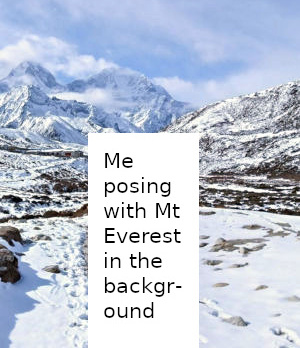
\includegraphics[width=\linewidth]{parts/general/picture.jpg}	%trimming relative to image size
%\includegraphics[width=\linewidth]{parts/general/anonpicture.jpg}	%trimming relative




%---------------------------------------------------------------------------------------
%	META SKILLS
%---------------------------------------------------------------------------------------

%---------------------------------------------------------------------------------------
%	WORK PHILOSOPHY
%---------------------------------------------------------------------------------------
\vfill\null

\cvsection{PHILOSOPHY}

\cvtext{``\mbox{Persevere through challenges}''}

\vfill\null

\input{generated/meta/\jobpos.tex}



%--------------------------------------------------------------------------------
%	EDUCATION
%--------------------------------------------------------------------------------

\vfill\null

\cvsection{EDUCATION}

\cvmetaevent
{}
{PhD Machine Learning\hfill\normalfont2019 - NOW}
{University1}
{Thesis title: "Fancy Title Here"}

\cvmetaevent
{}
{BSc Informatics\hfill\normalfont2009 - 2017}
{University2}
{Thesis title: "Fancy Title Here"}

\vfill\null

\cvsection{CONTACT}

\icontext{MapMarker}{12}{location}{black}\\[6pt]
\icontext{MobilePhone}{12}{+31 6 12345678}{black}\\[6pt]
\iconemail{Envelope}{12}{anon@anon.nl}{anon@anon.nl}{black}\\[6pt]
\iconlinkedin{Linkedin}{12}{linkedin.com/in/johndoe}{https://linkedin.com/in/johndoe}{black}\\[6pt]

\vfill\null
%\newpage

%\vfill\null
%\cvqrcode{0.7}

%\newpage

%----
% activities & hobbies
%----

%\cvsection{ACTIVITIES}
%\cvmetaevent{arg1}{arg2}{arg3}{arg4}

%\cvsection{ABOUT}
%\cvmetaevent{}{}{}{I am currently living in Rotterdam and my hobbies involve hiking, cooking and computing. I am currently training for a tour de mont blanc. A multiday hike around the mont blanc area.}

%\vfill\null
%\cvqrcode{0.7}

%\mbox{} % hotfix to place qrcode on the bottom when there are not other elements
%\vfill\null
%\cvqrcode{0.7}
%\newpage

\end{leftcolumn}
\begin{rightcolumn}
%---------------------------------------------------------------------------------------
%	TITLE  HEADER
%----------------------------------------------------------------------------------------
\fcolorbox{white}{darkcol}{\begin{minipage}[c][1.8cm][c]{1\mpwidth}
	\begin {center}
		\HUGE{ \textbf{ \textcolor{white}{ \uppercase{ Jan Jansen } } } } \\
		\large{ \textcolor{white} {Machine Learning Engineer} }
	\end {center}
\end{minipage}} \\[14pt]
\vspace{-12pt}


%---------------------------------------------------------------------------------------
%	PROFILE
%----------------------------------------------------------------------------------------
%\vfill\null
\vspace{.2cm}
\cvtext{As an ardent champion of machine learning, I am deeply committed to promoting the benefits of data-informed decision making and advocating for the significance of data. Concentrating on propelling achievement through insights derived from machine learning, I bring a wealth of experience in crafting strategies for data acquisition, analysis, and visualization, as well as fostering understanding of data and championing optimal practices. My fervor for leveraging machine learning to unearth fresh opportunities and optimize procedures has consistently resulted in triumphant outcomes and considerable enhancements for the organizations I've had the privilege to work with.}

%---------------------------------------------------------------------------------------
%	WORK EXPERIENCE
%----------------------------------------------------------------------------------------
\cvsection{EXPERIENCE}

\cvevent
{Jan 19 - NOW}
{PhD Candidate in Machine Learning for Medical Imaging}
{University1}
{Specializing in medical imaging analysis for novel diagnostics using state-of-the-art data science techniques and radiomics machine learning models, with a focus on head and neck carcinomas and degenerative disc disease in the neck.}
{\cvlist{
		\item Proficient in using PyTorch, NumPy, scikit-learn, SciPy, and XGBoost for developing and evaluating models for medical imaging research.
		\item Conducted research to develop innovative diagnostic tools for predicting therapy response and survival in patients with head and neck carcinomas, as well as for diagnosing degenerative disc disease in the neck.
		\item Developed and contributed to popular medical data science tools such as Tool1 and Tool2. Developed tools like Tool3 for detecting degenerative disc disease in the neck, and Tool4, a widely-used Python library.
		\item Supervised MSc. students in their thesis projects and served as a teaching assistant for Advanced Data Analysis with Python.
}}
{PyTorch · Scikit-Learn · XGBoost · NumPy · Pandas · Python · Git}


\cvevent
{Feb 20 - Dec 22}
{Founder of Company1}
{Self-Employed}
{As the founder of Company1, I established a platform that collects, processes, models, and presents <<Redacted>>-related data to the general public.}
{\cvlist{
		\item Awarded the RDNL Dutch Data Prize for <<Redacted>> for significant contributions to making <<Redacted>> data more Findable, Accessible, Interoperable, and Reusable.
		\item Design and maintenance of ETL and CI/CD pipelines, ensuring accurate and comprehensive data, as well as seamless integration and delivery for the platform.
		\item Developed models surpassing <<Redacted>>'s accuracy for vaccine rollout estimates and for estimating case counts using wastewater surveillance data.
		\item Developed the <<Redacted>> library, a transparent, open-source alternative to the government-released QR code app and library for the coronavirus passport.
}}
{Scikit-Learn · NumPy · Pandas · Python · Git · ETL}

\cvevent
{Aug 17 - Dec 18}
{Scientific Programmer}
{University1}
{Skilled scientific programmer with Python and data science expertise, excelling in infrastructure management, machine learning, high-performance computing, and Big Data analysis. Proficient in IaaS, Salt Project, and CI/CD practices, specializing in medical imaging and modeling solutions.}
{\cvlist{
		\item Contributed to <<Redacted>>, designing a system similar to Kubernetes Batch.
		\item Leveraged data science skills to develop efficient Python ETL pipelines, applying machine learning pipelines for predictive modeling and data analysis automation.
		\item Managed large-scale computational tasks using 3500+ CPU cores, demonstrating proficiency in IaaS platforms and HPC clusters.
		\item Utilized Flask, SQLAlchemy, NumPy, and Pandas for data manipulation, analysis, and visualization, aiding in data-driven decision-making.
		\item Showcased expertise in handling and organizing medical imaging data using XNAT and led innovative medical imaging projects.
		\item Employed CI/CD practices for seamless integration and deployment, and utilized Salt Project for scalable infrastructure management.
}}
{Data Pipelines · Big Data · Machine Learning · HPC Cloud · Medical Imaging · XNAT · IaaS · Salt Project · Python}

\cvevent
{Jan 17 - Jul 17}
{Intern}
{University1}
{Successfully completed my Bachelor's thesis: "Fancy Title 1"}
{}
{}
%{Batch Processing · Data Pipelines · Flask · Databases · SQLAlchemy · Python (Programming Language) · Object-Oriented Programming (OOP) · Git · JavaScript ·  Development}

\cvevent
{Jul 12 - Aug 16}
{Software Engineer}
{Company2}
{As a Software Engineer, my primary focus was on the continuous development and enhancement of the <<Redacted>> platform in the financial sector. This platform served as a vital communication channel between customers, banks, and intermediaries in the mortgage industry. }
{\cvlist{
		\item Orchestrated migration from a DIY server setup to cloud infrastructure, boosting scalability, reliability, and cost-efficiency.
		\item Developed on the <<Redacted>> platform and the advice module, creating automated mortgage advice based on user profiles and predictive algorithms.
		\item Enabled further integrations with the <<Redacted>> network. The software processed ~50\% of <<Redacted>> requests in the Netherlands during its peak.
		\item Implemented the SEPA transaction code for secure financial transactions.
		\item Championed the adoption of Agile methodologies, improving project delivery, client satisfaction, and fostering team collaboration.
		\item Pioneered the migration from Subversion to Git for source code repository, enhancing version control and code collaboration.
}}
{Scrum · Git · PHP · JavaScript · HTML · REST · MySQL}




%-----
% publications
%-----
%	Publications are optional in case the job / position requires it

\cvsection{PUBLICATIONS}

\nobibliography{parts/general/publications.bib}
\bibliographystyle{apacite}
\begingroup
\renewcommand{\section}[2]{}

\begin{thebibliography}{}
%	\item A list of publications
	\item \bibentry{pub1}
	\item \bibentry{pub2}
\end{thebibliography}
\endgroup

\newpage

% hotfixes to create fake-space to ensure the whole height is used
\mbox{}
\vfill
\mbox{}
\vfill
\mbox{}
\vfill
\mbox{}
\end{rightcolumn}
\end{paracol}


\let\clearpage\relax

\end{document}

